\begin{pastexam}[label={px:ntu-106-ie-ds-13}]{臺大工工所 106 學年度 第 13 題}
（複選；每題 10 分，每個選項單獨計分，答對 2 分，答錯倒扣 2 分）

Inserting nodes to a 2-3-4 tree with the following order using top-down insertion:
\{ 15, 14, 13, 12, 11, 10, 9, 8, 7, 6, 5, 4, 3, 2, 1 \}. Which of the following is(are) true?
\begin{enumerate}[label=(\Alph*),nosep]
\item The root node of the resultant tree is a 3-node.
\item There is only one 4-node in the resultant tree.
\item Numbers 9 and 10 are in the same node.
\item More than half of the nodes are 3-node.
\item If we insert a new number ``16'' to the tree, the height of the tree will be incremented by one.
\end{enumerate}
\end{pastexam}

\begin{pastsoln}
答案：(A)(B)。

由上而下的插入照資結書第~11.1.5~節（虛擬碼~11.1）：從根往下走，路上遇到 4-節點（3 個鍵）就先分裂，中間的鍵送進
父節點（根是 4-節點時中間鍵自己成為新根，樹長高一層）；走到葉子直接放進去。 下面用 $[\,\cdot\,]$ 表示一個節點，
「$\mid$」分隔同一層的節點。

\begin{center}
\small
\begin{tabular}{cl}
\toprule
插入 & 插入後的樹（由上往下每層一列） \\
\midrule
15, 14, 13 & $[13\ 14\ 15]$ \\
12 & 根是 4-節點，先分裂成 $[14]$；$12$ 放進左葉：$[14]$ / $[12\ 13] \mid [15]$ \\
11 & $[14]$ / $[11\ 12\ 13] \mid [15]$ \\
10 & 左葉是 4-節點，分裂，$12$ 上去：$[12\ 14]$ / $[10\ 11] \mid [13] \mid [15]$ \\
9 & $[12\ 14]$ / $[9\ 10\ 11] \mid [13] \mid [15]$ \\
8 & 分裂 $[9\ 10\ 11]$，$10$ 上去：$[10\ 12\ 14]$ / $[8\ 9] \mid [11] \mid [13] \mid [15]$ \\
7 & 根是 4-節點，分裂：$[12]$ / $[10] \mid [14]$ / $[7\ 8\ 9] \mid [11] \mid [13] \mid [15]$ \\
6 & 分裂 $[7\ 8\ 9]$，$8$ 上去：$[12]$ / $[8\ 10] \mid [14]$ / $[6\ 7] \mid [9] \mid [11] \mid [13] \mid [15]$ \\
5 & $[12]$ / $[8\ 10] \mid [14]$ / $[5\ 6\ 7] \mid [9] \mid [11] \mid [13] \mid [15]$ \\
4 & 分裂 $[5\ 6\ 7]$，$6$ 上去：$[12]$ / $[6\ 8\ 10] \mid [14]$ / $[4\ 5] \mid [7] \mid [9] \mid [11] \mid [13] \mid [15]$ \\
3 & 分裂 $[6\ 8\ 10]$，$8$ 上去：$[8\ 12]$ / $[6] \mid [10] \mid [14]$ / $[3\ 4\ 5] \mid [7] \mid \cdots$ \\
2 & 分裂 $[3\ 4\ 5]$，$4$ 上去：$[8\ 12]$ / $[4\ 6] \mid [10] \mid [14]$ / $[2\ 3] \mid [5] \mid [7] \mid \cdots$ \\
1 & $[8\ 12]$ / $[4\ 6] \mid [10] \mid [14]$ / $[1\ 2\ 3] \mid [5] \mid [7] \mid [9] \mid [11] \mid [13] \mid [15]$ \\
\bottomrule
\end{tabular}
\end{center}
插入 3 時，從根 $[12]$ 往下，要走的子節點 $[6\ 8\ 10]$ 是 4-節點，先分裂（$8$ 進根），再往下經過 $[6]$ 到葉子
$[4\ 5]$，放進去成為 $[3\ 4\ 5]$。 最後的樹：
\begin{center}
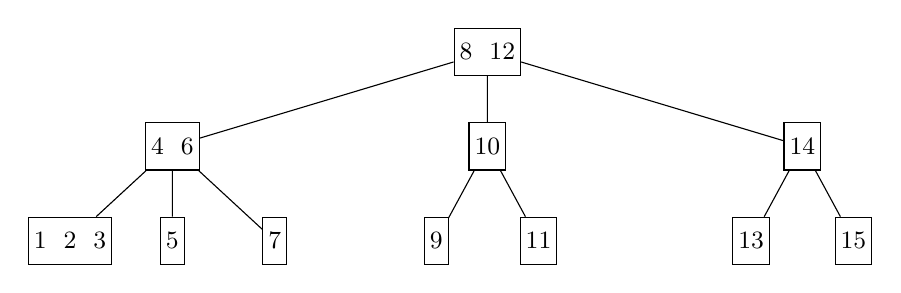
\begin{tikzpicture}[k/.style={draw,minimum height=6mm,inner sep=2pt,font=\small},
  level distance=12mm, level 1/.style={sibling distance=40mm}, level 2/.style={sibling distance=13mm}]
\node[k] {8\ \ 12}
  child {node[k] {4\ \ 6}
    child {node[k] {1\ \ 2\ \ 3}} child {node[k] {5}} child {node[k] {7}}}
  child {node[k] {10}
    child {node[k] {9}} child {node[k] {11}}}
  child {node[k] {14}
    child {node[k] {13}} child {node[k] {15}}};
\end{tikzpicture}
\end{center}
共 11 個節點：3-節點 2 個（$[8\ 12]$、$[4\ 6]$），4-節點 1 個（$[1\ 2\ 3]$），其餘 8 個是 2-節點；高度 3 層。

\textbf{逐項}：
\begin{itemize}
\item (A) 對。 根 $[8\ 12]$ 有 2 個鍵，是 3-節點。
\item (B) 對。 只有 $[1\ 2\ 3]$ 是 4-節點。
\item (C) 錯。 $9$ 在葉子 $[9]$，$10$ 在第二層的 $[10]$。
\item (D) 錯。 11 個節點裡只有 2 個 3-節點。
\item (E) 錯。 插入 16：根 $[8\ 12]$ 不是 4-節點，往右走到 $[14]$，再到葉子 $[15]$，路上都沒有 4-節點，直接放進葉子成為
$[15\ 16]$，沒有分裂，高度仍是 3。 樹只有在根是 4-節點而被分裂時才會長高。
\end{itemize}
\end{pastsoln}
